% !TeX root = ../../ZF_bmicha_Ana.tex
\subsection{Trägheitsmoment \hfill $I$}
    \subsubsection{2D}
        \textbf{Trägheitsmoment bzgl. einer Achse:}
        \begin{align*}
            I_x =& \iint_A \sigma(x,y) \cdot y^2 \, dA\\
            I_y =& \iint_A \sigma(x,y) \cdot x^2 \, dA
        \end{align*}
        \textbf{Polares Trägheitsmom.} (bzgl. $z$-Achse/ Ursprung):
        \begin{align*}
            I_o = I_x + I_y = \iint_A \sigma(x,y) \cdot (x^2 + y^2) \, dA 
        \end{align*}
        \textit{Keine Angabe für $\sigma$: $\sigma = 1$}

    \subsubsection{3D}
        \textbf{Trägheitsmoment bzgl. Achse:}
        \begin{align*}
            I_x =& \iiint_V \rho(x,y,z) \cdot (y^2 + z^2) \, dV\\
            I_y =& \iiint_V \rho(x,y,z) \cdot (x^2 + z^2) \, dV
        \end{align*}
        \textit{Keine Angabe für $\rho$: $\rho = 1$}
        
    \subsubsection{Satz von Steiner}
    \begin{minipage}{0.5\linewidth}
        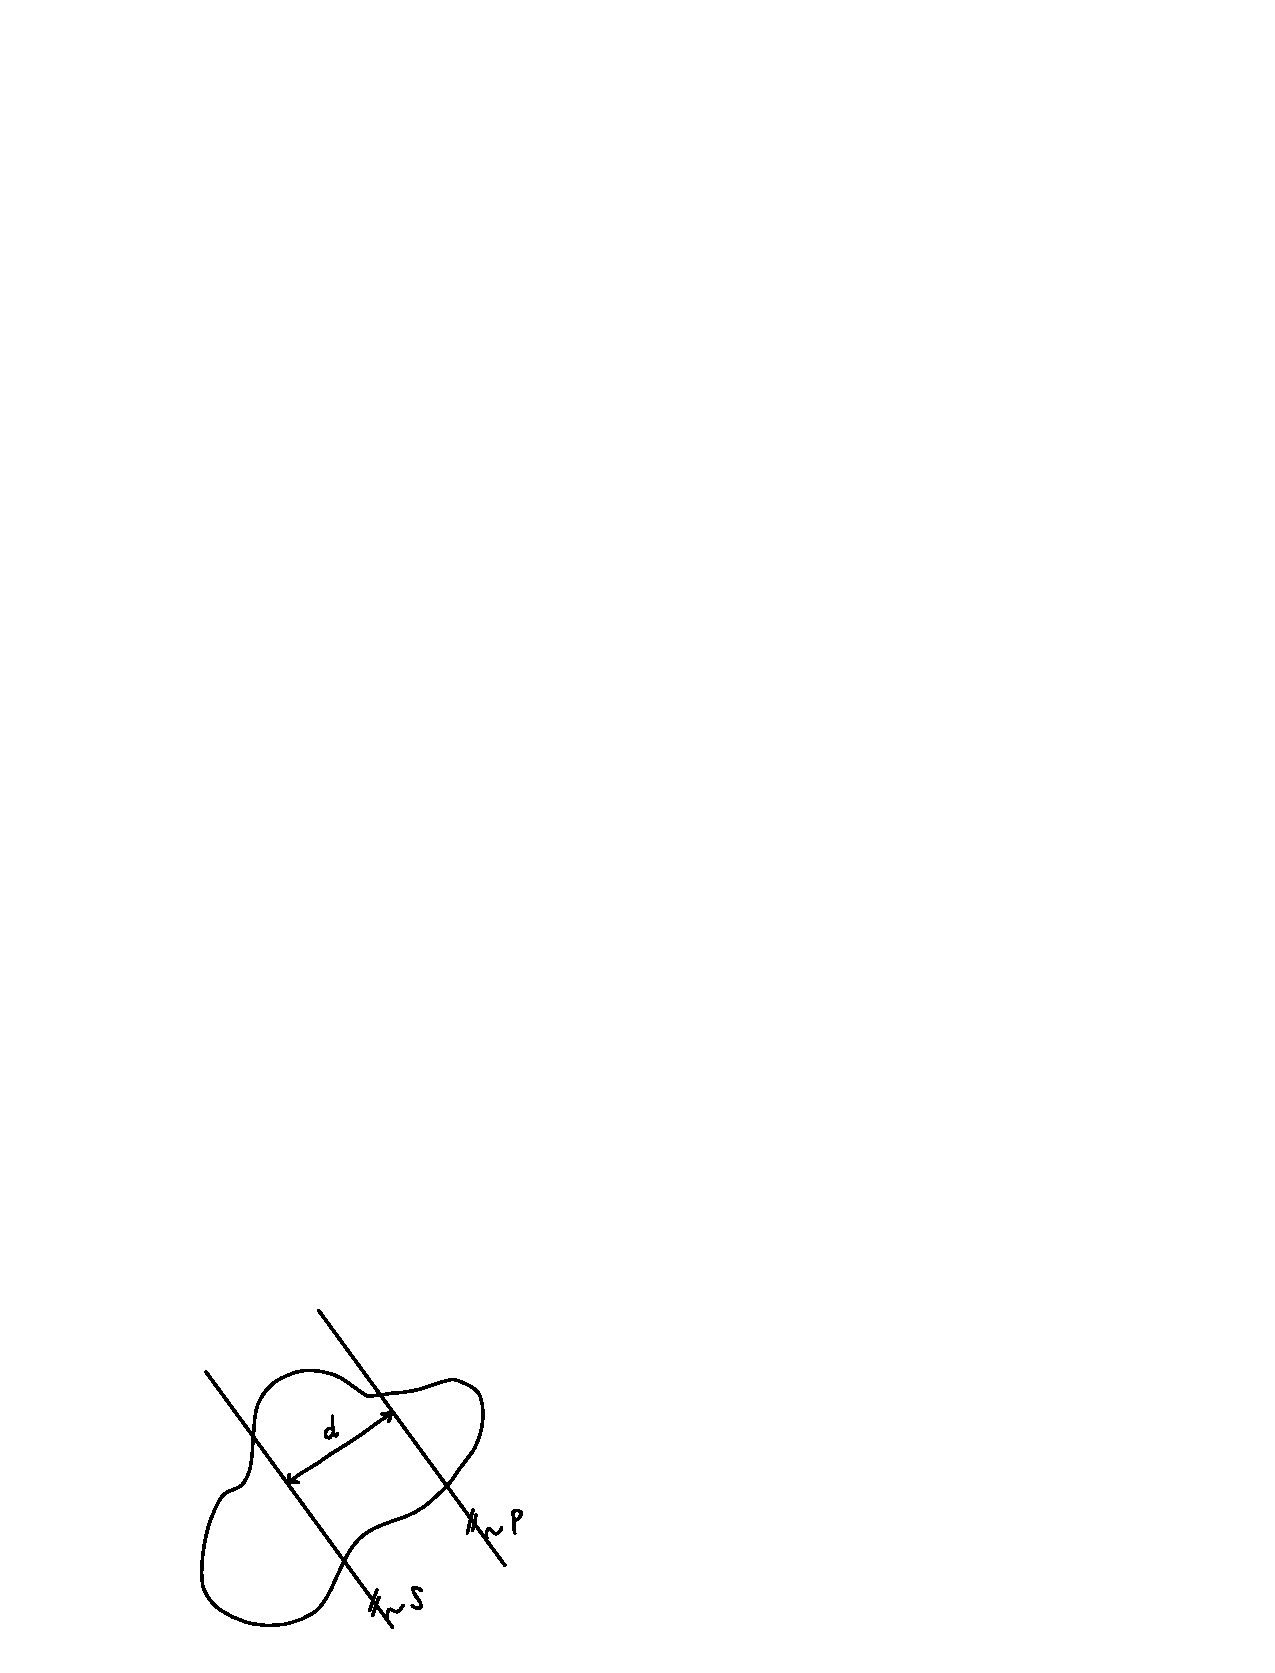
\includegraphics[width=\linewidth]{src/Mehrdimensionale-Funktionen_Integralrechnung/satz-von-steiner.pdf}
    \end{minipage}
    \hspace{0.05\linewidth}
    \begin{minipage}{0.4\linewidth}
        \begin{align*}
            I_p &=\,\, I_s + d^2 \cdot m\\
            m \vcentcolon&= Masse\\
            d \vcentcolon&= Abstand\\
        \end{align*}
    \end{minipage}